%!TEX root = ../Thesis.tex
\section{\glqq Was soll in die Cloud?\grqq~(An-Nam Pham)}
In Kapitel \ref{sec:IT-Infrastruktur} wurden die Vorteile für einen Umzug in die Cloud erläutert.
Da ein Teil der gesamten IT-Systemlandschaft (die zentrale Datenbank) innerhalb der Firma selbst betrieben wird, handelt es sich in diesem Fall um eine hybride Cloud, die aus der Private Cloud (zentrale Datenbank) und der Public Cloud besteht.\\
\\
Dieses Kapitel stellt unsere Empfehlung dar, was für Systeme (z.B. Module, Komponenten, etc.) in die Public Cloud installiert werden soll und was für ein Nutzen diese Systeme für das Unternehmen Stylez hat.
Die folgende Abbildung zeigt die empfohlene Implementierung der gesamten IT-Systemlandschaft. Die einzelnen Komponenten werden in den nächsten Unterkapiteln erläutert:
\begin{figure}[H]
\centering
\begin{minipage}[t]{0.8\textwidth}
\fbox{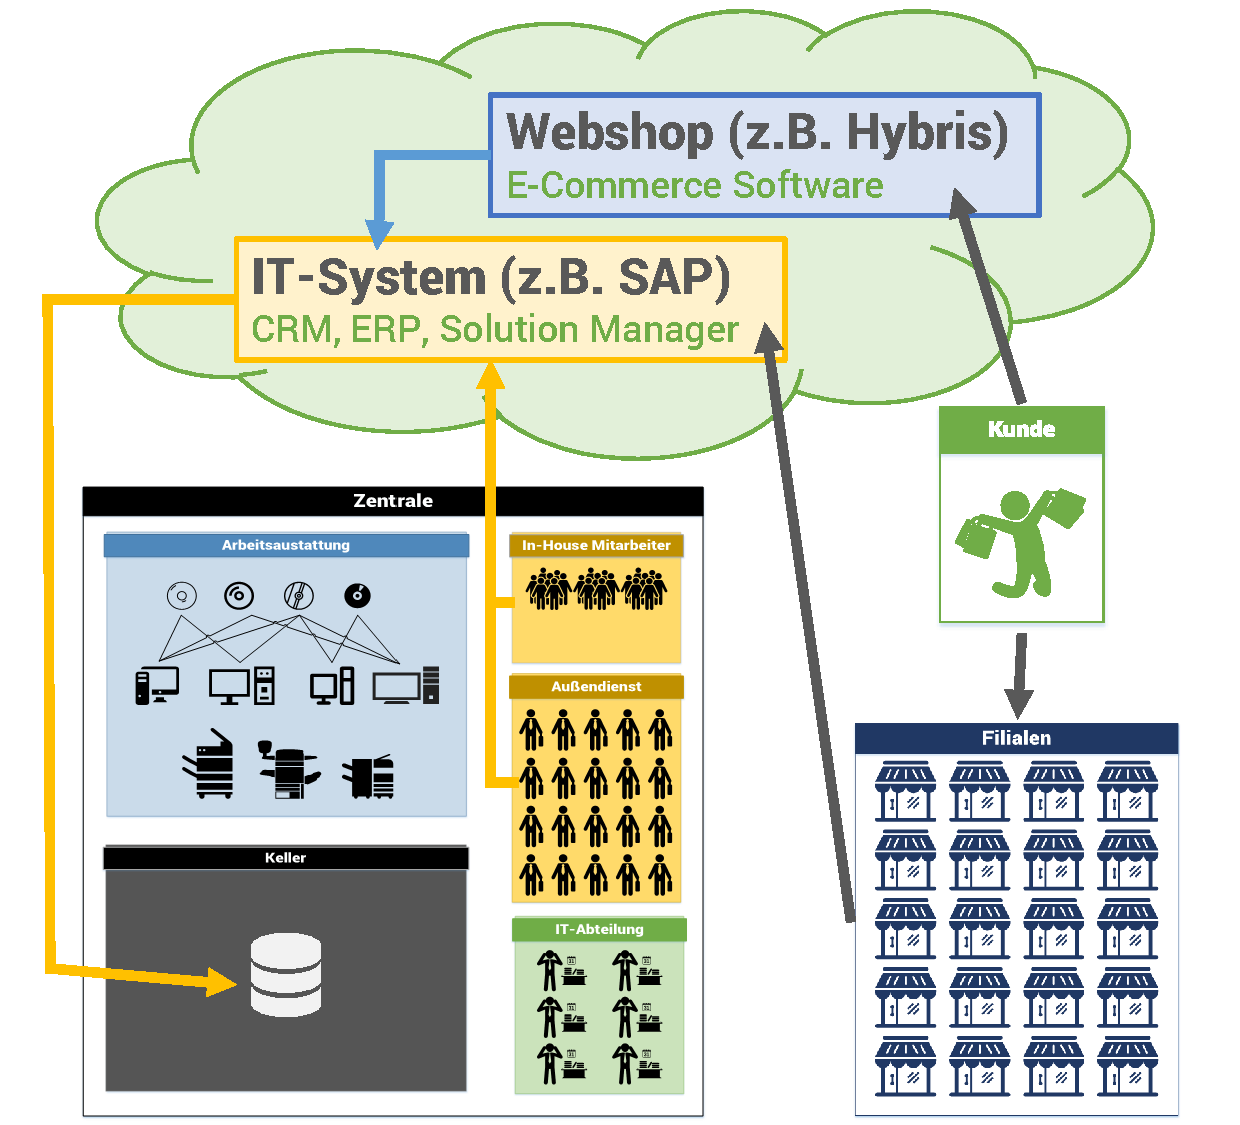
\includegraphics[width=1\textwidth]{img/Cloudinhalt.pdf}}
\caption{Empfohlene Implementierung der Hybrid Cloud} % Überschrift
\source{Eigene Darstellung} % Quelle
\label{img:Cloud_Implementierung}
\end{minipage}
\end{figure}
\subsection{SAP IT-System}
Wir empfehlen die gesamte Unternehmensstruktur von Stylez mit Hilfe von SAP im IT-System abzubilden\footnote{Berechtigungskonzept, Organisationsmanagement, Geschäftsprozesse, etc. werden in SAP ERP abgebildet, um ein optimales Business-IT-Alignment zu ermöglichen.}. Der Entscheidung für SAP bietet unter anderem folgende Vorteile\footcite{SAP_Vorteil}:
\begin{itemize}
\item Internationaler Anbieter
\item führende Technologie
\item 40 Jahre Erfahrung mit kfm. Software
\item technische Innovationskraft
\item finanzielle Stabilität
\end{itemize}
Außerdem gibt es viele SAP-Partner, die auf den Fashion-Handel spezialisiert sind. Diese haben unter anderem folgende Stärken:
\begin{itemize}
\item Kundennähe
\item Mittelstandsausrichtung und -erfahrung
\item Angebot als Generalunternehmer
\end{itemize}
Das SAP System soll aus ein \acrshort{ERP}-System, \acrshort{CRM}-System und einen Solution Manager bestehen.
\subsubsection{SAP ERP}
Das \acrlong{ERP}-System (ERP-System) bildet (im Idealfall) das Unternehmen in seiner Gesamtheit zeitnah ab. Dadurch ist es ein sehr wertvolles Hilfsmittel für Planungs- und Steuerungsaufgaben, das unter anderem noch folgende Vorteile bietet:
\begin{itemize}
\item Erhöhte Automatisierung für kürzere Bearbeitungszeiten und Kostenersparnisse
\item Verringerte Durchlaufzeiten von Prozessen
\item Erhöhte Datenqualität, Redundanzen und Inkonsistenzen werden vermieden
\item Verbesserte Zusammenarbeit über Abteilungsgrenzen hinweg
\item Optimierter Informationsfluss im Unternehmen
\item Überwinden organisatorischer und technischer Schnittstellen
\end{itemize}
\underline{\textbf{Der große Nutzen:}}\\
ERP-Systeme tragen langfristig zur Leistungssteigerung und Kostenreduzierung bei, da das ERP-System sämtliche Bereiche wie z.B. Materialwirtschaft, Finanz- und Rechnungswesen, Personalwirtschaft, Verkauf, Marketing und Forschung abbildet. Dadurch können alle Bereiche miteinander kommunizieren und dieselbe Datenbasis nutzen. Dies spart z.B. im Vergleich zur \glqq Zettelwirtschaft\grqq~und Excel viel Zeit und Kosten.\footcite[vgl.][]{ERP}
\subsubsection{SAP CRM}
\glqq Der Kunde ist König\grqq. Dieser bekannte Satz drückt ganz gut aus, worauf man in einem Unternehmen ganz besonders achten muss.\\
Das \acrlong{CRM} (CRM) (zu Deutsch: Kundenbeziehungsmanagement) unterstützt das Unternehmen dabei, die Beziehung zu bestehenden und potenziellen Kunden zu verwalten und zu gestalten.\\
\\
\underline{\textbf{Der große Nutzen:}}\\
Das CRM-System verwaltet nicht nur bestehende und potenzielle Kunden des Unternehmens. Wird das Supply-Chain-Management eingebunden, kann das CRM-System auch Lieferanten verwalten. Im Fall von Stylez können auch alle Franchisenehmer eingebunden werden.\\
Das Besondere am CRM-System ist, dass es die Historie der Kundeninteraktion verfolgbar macht. Es kann sehr schnell ein Überblick über einen Kunden, Lieferanten oder Franchisenehmer\footnote{Zur Vereinfachung werden Kunden, Lieferanten oder Franchisenehmer im Folgenden mit Kunde zusammengefasst.} geschaffen werden (z.B. getätigte Anrufe, Häufigkeit der Support-Anfragen, Anteil am Geschäftsumsatz, uvm.).
Dadurch kann schnell auf den Kunden eingegangen. Dies spart Zeit und fördert die Professionalität und somit auch das Vertrauen der Kunden. Außerdem kann das CRM-Systen benutzt werden, um Prognosen über zu erwartende Ergebnisse einfacher und genauer zu erstellen. Und es bietet volle Transparenz und bei Bedarf jederzeit Zugriff auf Kundeninformationen.

\subsubsection{SAP Solution Manager}
sdfjkl
%SAP Rapid Deployment Solution
\subsection{Hybris (Webshop)}
\section{So funktioniert der Umzug in die Hybrid Cloud (An-Nam Pham)}
% \section{Stichwort: Hochverfügbarkeit}
\section{Roadmap (An-Nam Pham)}
